\chapter{Software of the Vision Correction Display}

\section{Introduction to Algorithms}

% Mention more about what Huang did later
Fu-Chun Huang et al. applied light field technology to develop an algorithm that created a sharp image on the display plane \cite{Huang:EECS-2013-206}. Peter Wu introduced the forward method and its optimizations \cite{Wu:EECS-2016-67}. Another new algorithm we will introduce is the backward method, which processes an image under the assumption that most light rays that travel through the center of the pinhole or lenslet. The method aims to improve run time compared to Huang's algorithm while taking into consideration more light rays than the forward method. We will use the same definitions, symbols, and content on Huang's algorithm and the optimized forward method in chapter 4 of Wu's paper \cite{Wu:EECS-2016-67} for consistency.

\subsection{Projection and Prefiltering}

Each algorithm in this paper is divided up into two components: the projection relationship and prefiltering. The projection relationship is the mapping relationship from a point on the display \footnote{To avoid confusion, display in this chapter means the phone screen and not the light field display. In later chapters, we will use the word screen instead of display.} to a point on the sensor or retina. The projection relationship depends on the experimental settings such as focal point, object focus, and object distance. Prefiltering is the step in which the content on the display is modified. Prefiltering takes in the projection relationship and the input image and produces a transformed output image.

\subsection{Symbols}

\begin{figure}[ht]
  \centering
  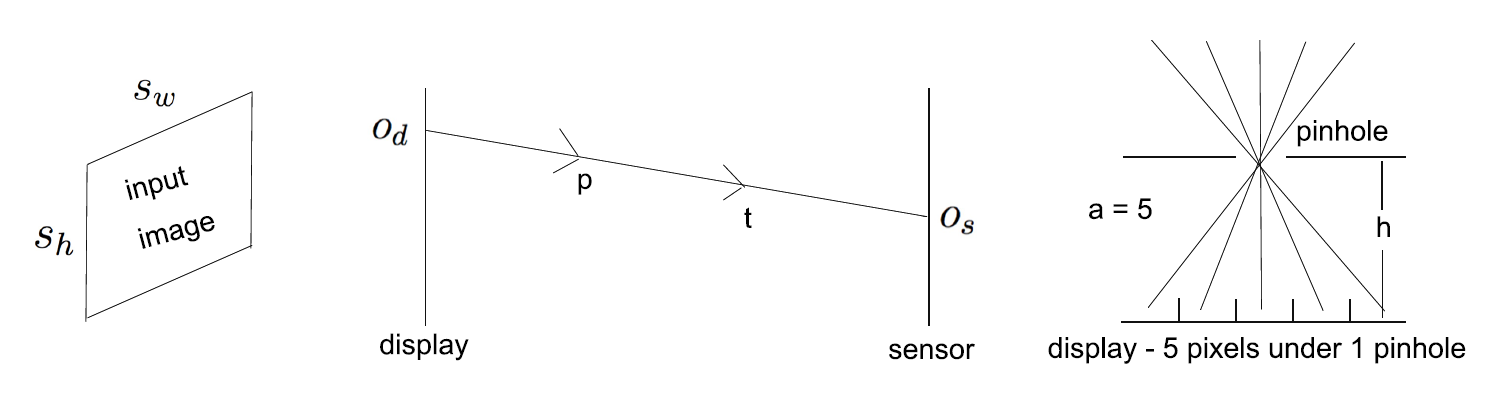
\includegraphics[width=5.0in]{chapters/chapter4/images/Prefilter.png}
  \caption{The figure shows the setup for the prefiltering algorithm. (left) The input image has dimensions $s_w$ by $s_h$ pixels. (middle) $p$ and $t$ are points on the light ray. (right) There are $5$ pixels under each pinhole, and $h$ is the distance between the pinhole and the display. This image is from \cite{Wu:EECS-2016-67}.}
  \label{fig:fr}
\end{figure}

The size of the input image is $s_w$ by $s_h$ pixels. The input image is the unmodified image a normal person sees on the display.
We define two functions $f_s$ and $f_d$, both of which contain the same parameters:
\begin{itemize}
\item $p$ and $t$ stand for arbitrary points in 3-D space. $p$ and $t$ specify a light ray.

\item $e$ is the experimental settings. If we only consider defocus (myopia or hyperopia), the only parameter to consider is the distance from the the screen to the lens.

\item $c$ is the condition of the camera or human eye. If we only consider defocus, then this parameter is the distance from the sensor to the lens.

\end{itemize}

$f_s$ takes in the parameters and computes the position $o_s$, the position where the light ray $(p,t)$ hits the sensor. Similarly, $f_d$ takes in the same parameters and computes the position $o_d$, the position where the light ray $(p, t)$ hits the display. \\
$$f_s(p, t, e, c) \rightarrow o_s$$
$$f_d(p, t, e, c) \rightarrow o_d$$
The functions $m_s$ and $m_d$ transforms an arbitrary position into a discrete two-dimensional index. Both take a parameter $p$ which is any point on either the display plane or sensor place and transform $p$ into a integer two-dimensional index. 
$$m_s(p) \leftarrow (a_s, b_s)$$
$$m_d(p) \rightarrow (a_d, b_d)$$
The angular resolution $a$ is the ratio of the screen resolution to that of the pinhole mask or lens array. If a 5x5 pixels are covered under the light field display, then $a = 5$ for the device.\\
The depth $h$ is the distance from the surface of the light field display to the plane of the phone display.

\section{Huang's Light Field Algorithm}

The projection relation is represented as a matrix in Huang's algorithm. He assumes that the sensor has the same resolution as that of the pinhole mask, which is $L_s = s_w / a$ by $L_d = s_h / a$. These display pixels have resolution $s_w$ $\times$ $s_h$. 
Next, the algorithm builds a projection matrix. First, an all-zero matrix $P$ with dimensions $L_d$ by $L_s$ is created. Second, for every pixel on the screen, n points $\{o_n\}$ are sampled on the aperture, and a light ray $p_s - o_i$ is constructed for each sample point. Third, the algorithm applies the function $f_d$ to get the position $p_d$ on the display. The function $f_d$ in this case uses Zernike polynomials and can consider higher order aberrations. Then, the function $m_d$ is called to convert $p_d$ into a 2-D index $I_d$. Finally, the algorithm adds index $I_d$ of the matrix by $1/n$. 

After the projection matrix is formed, the following linear equation needs to be solved, where $P$ is the project matrix and $b$ is the one-dimensional representation of the input image:

$$P \cdot x = b$$

$P$ is not a square matrix, but we can multiply both sides by $P^{T}$, and $P^{T}P$ is square.

$$(P^T \cdot P) \cdot x = p^T \cdot b$$

Define $H = P^T \cdot P$. There is a high chance that $H$ is singular and there is no solution to the linear system. To solve the linear system, a very small positive value $\lambda$ is defined and added to the the system where $I$ is the identity matrix:

$$H' \leftarrow H + \lambda \cdot I$$

$\lambda$ introduces a negligible amount of error to the system, and $H$ is not singular anymore.

Instead of solving the system directly, Huang's algorithm changes it into an optimization problem: \\
% Cite where Huang got his algorithm

$$\textbf{Minimize:} (H'x - P^Tb)^T \cdot (H'x-P^Tb)$$

The L-BGFS method \cite{Liu1989} was used to solve this optimization problem. The final result $x$ may have very large positive or very small negative values, but Huang cut off all values in the range (0, 255). The algorithm was applied for the R, G, and B (red, green, and blue) channels separately. The projection matrix was the same for computing the display matrix for each channel.

\subsection{Analysis}
Huang's algorithm is the most thorough algorithm in that it considers light rays for all possible positions on the aperture and therefore almost all possible positions between the display and sensor. However, it is subject to many flaws. The algorithm can lead to inconsistency if the number of random aperture samples is not large enough. It also has a slow runtime: the algorithm takes 45 seconds in MATLAB assuming the projection matrix for a viewing angle (angle between normal of phone display and sensor plane) of 0 was precomputed and roughly three hours if all viewing angles from -5 degrees to 5 degrees are considered. The time complexity of the algorithm is $\mathcal{O}(m \cdot n^2)$, where $m$ is the number of samples on the aperture and $n$ is the length of a square sensor. The algorithm leads to loss of light because it to divides by $n$ while most of the $n$ light rays do not reach the display. The assumption that the sensor resolution is $1/a$ that of the original display is misleading because a human eye often has resolution even better than that of the display. The algorithm ignores the pixel arrangements and the fact that each point on the display can only correspond to one color. Finally, the L-BGFS method makes the prefiltering speed greatly dependent on experimental settings and the user's eye condition and adds significant complexity to the algorithm.

\section{Forward Method}

In the forward method, we assume that the sensor has the same resolution as the display or screen, so if the display or phone screen has size $640 \times 640$ pixels, then so does the sensor. In addition, the light rays travel from the display to the sensor instead of from the sensor to the display.

In the projection step of the algorithm, we compute all possible relationships from each point on the display to any point on the sensor. Following the function $f_s$, the light ray travels in a continuous straight line from the display pixel $p_d$ to the center of the closest pinhole $o_c$, and if not blocked by the aperture, to a point on the sensor $o_s$. We keep track of the sensor position for each display position, and apply this process for the R, G, and B channels separately. Since the three channels occupy different positions on the display pixel\footnote{More on this will be covered in chapter 7. A pixel is composed of a red, green, and blue area.}, the list of sensor positions for each channel is different. Unlike Huang's algorithm, there are no matrices involved in the optimized forward method.

In prefiltering, the first step in is to the set the sensor image equal to the original perfect image. Then, for each display position $o_d$, we set its R, G, and B equal to pixel values at the precomputed sensor positions $o_s(R)$, $o_s(G)$, $o_s(B)$, respectively. The display color is set to $0$ if the sensor position is invalid.

The two steps can be merged together in that for each display pixel, the corresponding R, G, and B sensor pixel positions are computed and the display pixel colors is set to the sensor pixel colors. 

\lstset {language=C++}
\begin{lstlisting}[frame=single, basicstyle=\footnotesize\ttfamily, columns=fullflexible, caption=Pseudocode For Forward Method \protect\footnote{The R, G, and B channels are ignored for simplicity.}]
int[][] sensor_image = origin_image;
int[][] prefiltered_image = new int[sensor_image.height][sensor_image.width];
// Assume sensor_image is a square
int screen_size = sensor_image.width;
int aperture_radius = 0.003; // 3 mm aperture radius

// Loop through the display image
for (int y_index = 0; y_index < screen_size; y_index++) {
  for (int x_index = 0; x_index < screen_size; x_index++) {
    float2 screen_pos = compute_screen_pos(x_index, y_index);
    float2 pinhole_pos = find_nearest_pinhole(screen_pos);
    float2 aperture_pos = compute_aperture_pos(screen_pos, pinhole_pos);
    if (aperture_pos.norm < aperture_radius) {
      int2 sensor_pos = ray_trace(screen_pos, pinhole_pos, sensor_image);
      prefiltered_image[screen_pos] = sensor_image[sensor_pos];
    }
  }
}
\end{lstlisting}
\footnotetext{The R, G, and B channels are ignored for simplicity.}

\subsection{Analysis}
The mains benefits of the forward method are that it is fast and simple. The method has a run time of less that one second for large images and a time complexity of $\mathcal{O}(n^2)$, a major improvement over Huang's algorithm. Huang's algorithm samples many rays that are blocked by the pinhole mask, while the forward method ignores such samples. One issue with the forward method is that only light rays that travel through the center of the pinhole mask are considered, which could lead to loss of information. In addition, by starting from the display, the amount of light a sensor pixel receives is hard to measure.

\section{Backward Method}

In the backward method, rays are traced from the sensor to the screen, like in Huang's algorithm. We also assume that the resolution of the display and the sensor are the same. 

In the projection step of the algorithm, we compute all possible points on the display for each point on the sensor. The function $f_d$ applies Gaussian ray tracing, where the sensor pixel $p_s$ corresponds to a point on the focus plane $o_f$, and we check whether a ray traveling from $o_f$ in the direction of $o_c$ is blocked by the aperture or pupil. If not blocked, the intersection of the ray and display plane $o_d$ is added to the list of display points for the sensor pixel. $f_d$ is applied for every pinhole. The RGB channels are not taken into consideration to make sure that the number of red, green, and blue hits are equal. Like the forward method, there are no matrices involved, although it is possible for generate the projection in matrix form.   

In prefiltering, the first step is to the set the sensor image equal to the original perfect image, the display image equal to a $s_w \times s_h$ array of zeros, and a counter matrix of size $s_w$ by $s_h$ for normalization. For each sensor pixel $p_s$, we check the set of display pixels from projection $\{p_d\}^n$ and increment the color of the display pixel $p_d$ is by the the color on the sensor pixel $p_s$ and the temporary matrix at $p_d$ by 1. We then do a matrix pointwise division between the display image and the counter matrix.

The two steps can be merged together in that for each sensor pixel, the corresponding display positions for each pinhole are computed and the display pixel colors are set to the sensor pixel colors. 

\begin{lstlisting}[frame=single, basicstyle=\footnotesize\ttfamily, columns=fullflexible, caption=Pseudocode For Backward Method \protect \footnote{The R, G, and B channels are ignored for simplicity.}]
int[][] sensor_image = origin_image;
int[][] prefiltered_image = new int[sensor_image.height][sensor_image.width];
int[][] prefiltered_image_norm = new int[sensor_image.height][sensor_image.width];
// Assume sensor_image is a square
int sensor_size = sensor_image.width;
int angular_resolution = 5;
int pinhole_size = sensor_size // angular_resolution
int aperture_radius = 0.003; // 3 mm aperture

// Loop through the sensor image
for (int y_index = 0; y_index < sensor_size; y_index++) {
  for (int x_index = 0; x_index < sensor_size; x_index++) {
  int2 screen_pos = (x_index, y_index)
    // Check each pinhole
    for (int py = 0; py < pinhole_size; py++) {
      for (int px = 0; px < pinhole_size; px++) {
        float2 pinhole_pos = compute_pinhole_pos(px, py);
        float2 aperture_pos = compute_aperture_pos(pinhole_pos, screen_pos);
        if (aperture_pos.norm < aperture_radius) {
          float2 display_pos = compute_display_pos(pinhole_pos, aperture_pos);
          prefilter_image[display_pos] += sensor_image[screen_pos];
          prefilter_image_norm[display_pos] += 1;
        }
      }
    }
  }
}

for (int y_index = 0; y_index < sensor_size; y_index++) {
  for (int x_index = 0; x_index < sensor_size; x_index++) {
    int2 screen_pos = (x_index, y_index);
    prefilter_image[screen_pos] /= prefilter_image_norm[screen_pos];
  }
}
\end{lstlisting}
\footnotetext{The R, G, and B channels are ignored for simplicity.}

\subsection{Analysis}
The backward method seeks to fix some issues of both Huang's algorithm and the forward method, but also has issues similar to both. It is simpler than Huang's algorithm but more complex than the forward method. The method takes around 2.5 minutes to run, which is better that Huang's algorithm at multiple angles and slower than both the one angle version of Huang's algorithm and the forward method. The time complexity is $\mathcal{O}(n^4)$, which is worse that Huang's algorithm for large screen sizes. There is a lot of unnecessary sampling as light from many pinholes will not reach a specific point on the sensor. Like the forward method, only light rays that travel through the center of the pinhole mask are considered, which could lead to loss of information. One way to reduce this loss of information is to take many samples points on the sensor pixel, but this makes the run time even worse. The main benefits of the backward method are that it is most similar to the software simulation algorithm and that light passing through every pinhole is considered for each sensor pixel. 

% confusing position and pixel
% Insert images here
% In the future, consider the one-to-one and many-to-many relationship, it is still confusing for many group members